\documentclass{handout}

\SetInstructor{Lt Col James Phillips}
\SetCourseTitle{ECE231: Electrical Circuits and Systems I}
\SetSemester{Spring 2016}
\SetHandoutTitle{Lecture 9: Thevenin and Norton Equivalent Circuits}
%\SetDueDate{1 Jan 2016}
%\ShowAllBlanks

\showsoln \setsolncolor{red}

\begin{document}
\maketitle

\textbf{Upcoming events}
\begin{enumerate}
\item HW \#3 due next lesson
\item Problem set \#2 due next lesson
\item Quiz \#2 next lesson
\item Block 2 Skills Review due Lesson 14
\end{enumerate}

\textbf{OBJECTIVES:}
\begin{enumerate}
\item Demonstrate the ability to find Thevenin and Norton equivalent circuits
\item Demonstrate the ability to analyze circuits using Thevenin/Norton equivalent sources
\end{enumerate}

\textbf{READING}
\begin{description}
\item [Required]:
\begin{itemize}
\item  Textbook, sections 3.4, pages 109--119
\end{itemize}
\item [Optional]: None
\end{description}

\textbf{HOMEWORK}
\begin{description}
\item [Required textbook problems]: 3.47, 3.49, 3.51 --- Due Lesson 10
\item [Recommended textbook problems]: 3.56, 3.57
\end{description}

\section{Statement of Thevenin's and Norton's Theorems}
\subsection{Some Preliminary Definitions}
\soln{3in}{
\begin{description}
\item[Interface] -- a connection between two circuits; for our purposes this is normally a two terminal interface
\item[Source Circuit] -- Notionally, the portion of the circuit that provides a signal to the remaining circuit; however, in this context it is really just the portion of the circuit that we will replace with an equivalent circuit.  For the theorems to apply, the source circuit must be linear.
\item[Load Circuit] -- Notionally, the portion of the circuit that is consuming power from the source circuit.  In this context, it is what ever remails after we have identified our ``source'' circuit.
\end{description}

}
\begin{figure} [h t b]
\centering
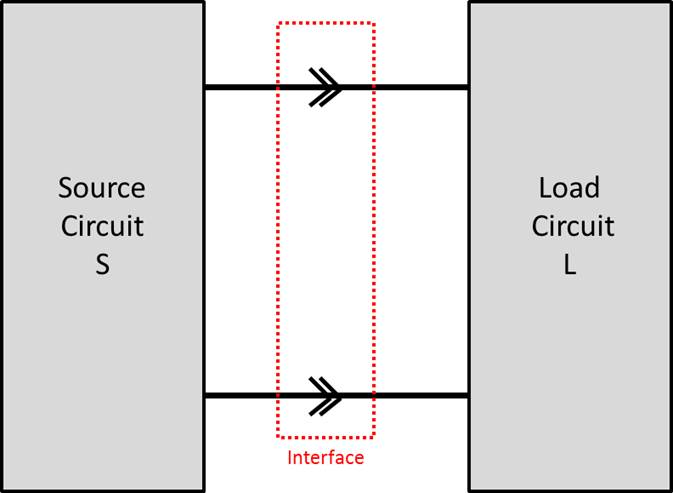
\includegraphics[width=0.4\textwidth]{Definitions.jpg}
\caption{Reference for definitions}
\label{fig: Definitions}
\end{figure}

\subsection{Statement of Thevenin's Theorem}
Thevenin's theorem simply states that the entire source circuit can be replaced with an independent voltage source ($v_T$) in series with a single resistor ($R_T$).  When this replacement is done, there is no change to the $i$--$v$ relationship at the source--load {\em interface}. A  Thevenin equivalent circuit is shown in Figure \ref{fig: Thevenin_Norton}(a).

\begin{figure} [h t b]
\centering
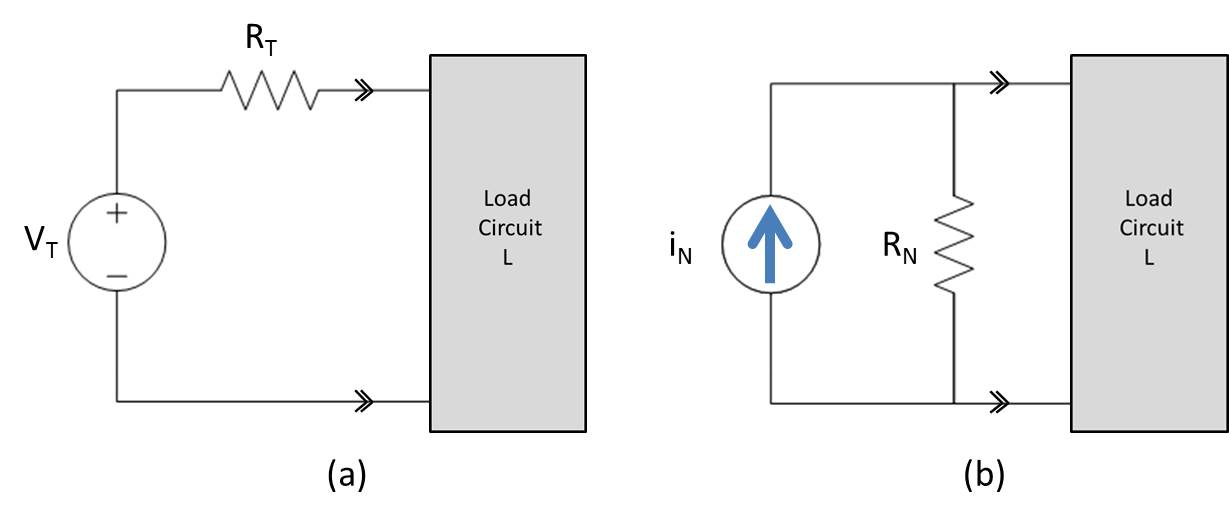
\includegraphics[width=0.7\textwidth]{Thevenin_Norton.jpg}
\caption{(a) Thevenin and (b) Norton Equivalent Circuits}
\label{fig: Thevenin_Norton}
\end{figure}

\subsection{Statement of Norton's Theorem}
Norton's theorem simply states that the entire source circuit can be replaced with an independent current source ($i_T$) in parallel with a single resistor ($R_T$).  When this replacement is done, there is no change to the $i$--$v$ relationship at the source--load {\em interface}.  A  Norton equivalent circuit is shown in Figure \ref{fig: Thevenin_Norton}(b).



\subsection{Another important note}
Since both the Thevenin Circuit and the Norton Circuit have identical $i$--$v$ (at the interface) to the original circuit, they have identical $i$--$v$ relationships to one another (also at the interface).

\section{Finding the Thevenin or Norton Equivalent Circuit}
How do we go about finding the values of our sources and resistances for the our Thevenin or Norton circuits?

\textbf{To find a Thevenin voltage,} you simply replace the load with an open circuit and find the open circuit voltage, $v_{oc}$; see Figure \ref{fig: v_oc_i_sc}(a). Then,
\soln{1in}{
\begin{equation}
v_T=v_{oc}
\end{equation}
}
\begin{figure} [h t b]
\centering
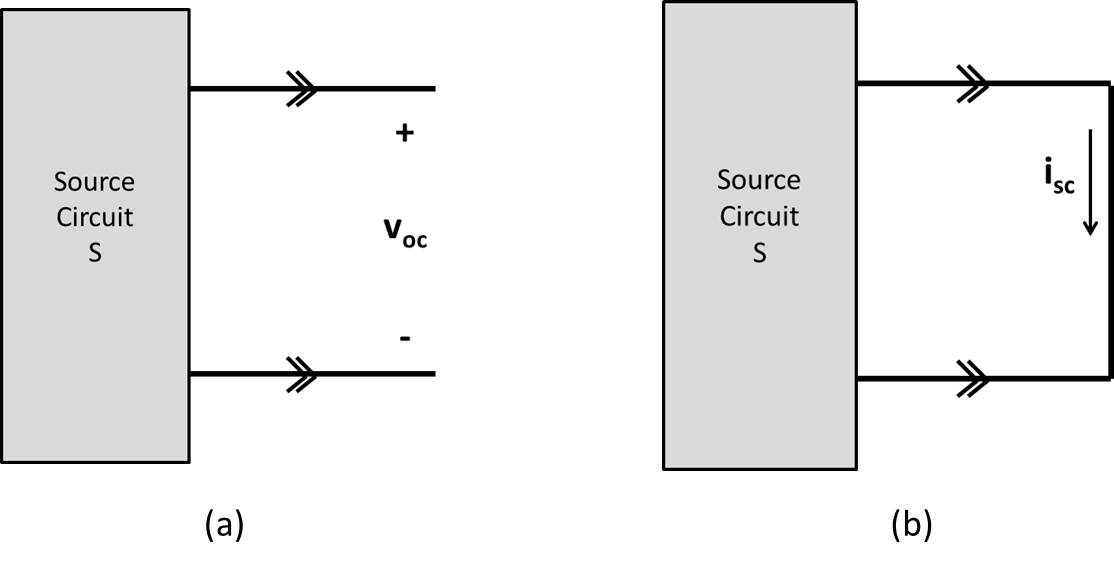
\includegraphics[width=0.7\textwidth]{v_oc_i_sc.jpg}
\caption{Finding (a) Thevenin Voltages and (b) Norton Currents}
\label{fig: v_oc_i_sc}
\end{figure}

\textbf{To find a Norton current,} you simply replace the load with a short circuit and find the short circuit current, $i_{sc}$; see Figure \ref{fig: v_oc_i_sc}(b). Then,
\soln{1in}{
\begin{equation}
i_N=i_{sc}
\end{equation}
}


\textbf{To find the Thevenin Resistance,} there are two methods.  The first is to find both $v_T$ and $i_N$ and use
\soln{1in}{
\begin{equation}
R_T=R_N=\frac{v_{oc}}{i_{sc}}=\frac{v_T}{i_N}
\end{equation}
}

The other method is called {\em look-back}. To utilize the look-back method, we short the voltage sources and open the current sources in the \textbf{source circuit}.  With then calculate the resistance of this new circuit (with the load disconnected).  This will give us our $R_T$; thsi will be demonstrated in some of our examples below.

\newpage
\clearpage
\pagebreak

\section{Examples}

\subsection{Example 1 - Textbook Exercise 3-28}
Find the Thevenin equivalent of the circuit shown in Figure \ref{fig: Example1}.  Then find the Norton Equivalent.
\begin{figure} [h t b]
\centering
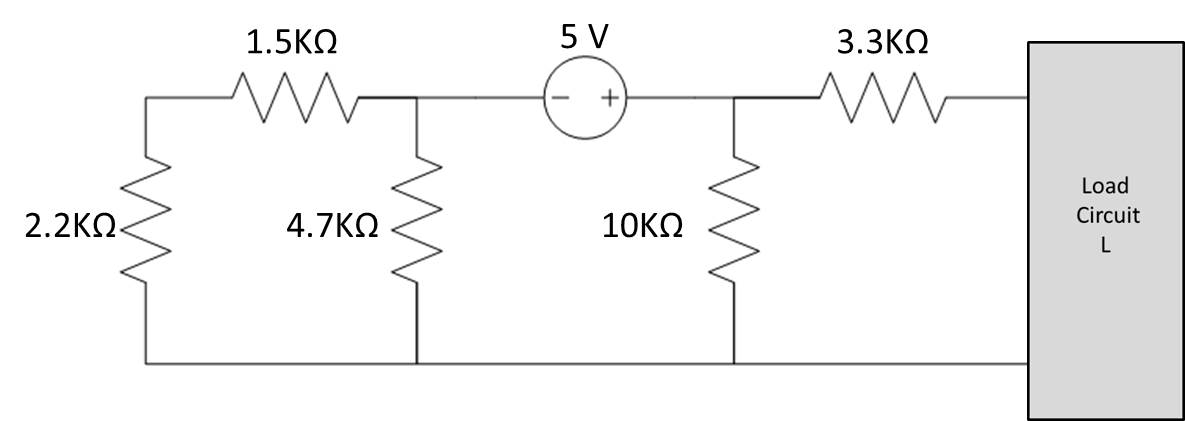
\includegraphics[width=0.7\textwidth]{Example1.jpg}
\caption{Example 1 Circuit}
\label{fig: Example1}
\end{figure}

\soln{6in}{
\begin{figure} [h t b]
\centering
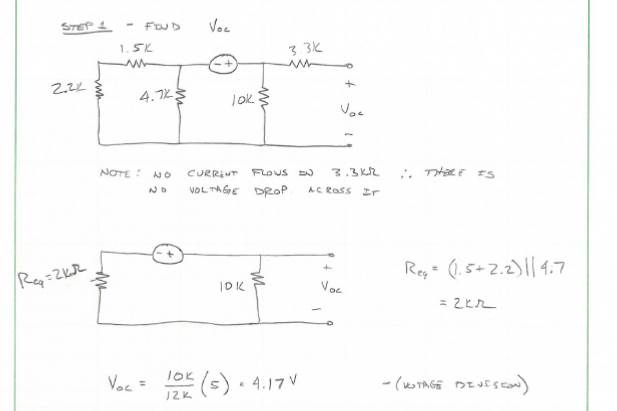
\includegraphics[width=0.9\textwidth]{Example1solnA.jpg}
\end{figure}

\begin{figure} [h t b]
\centering
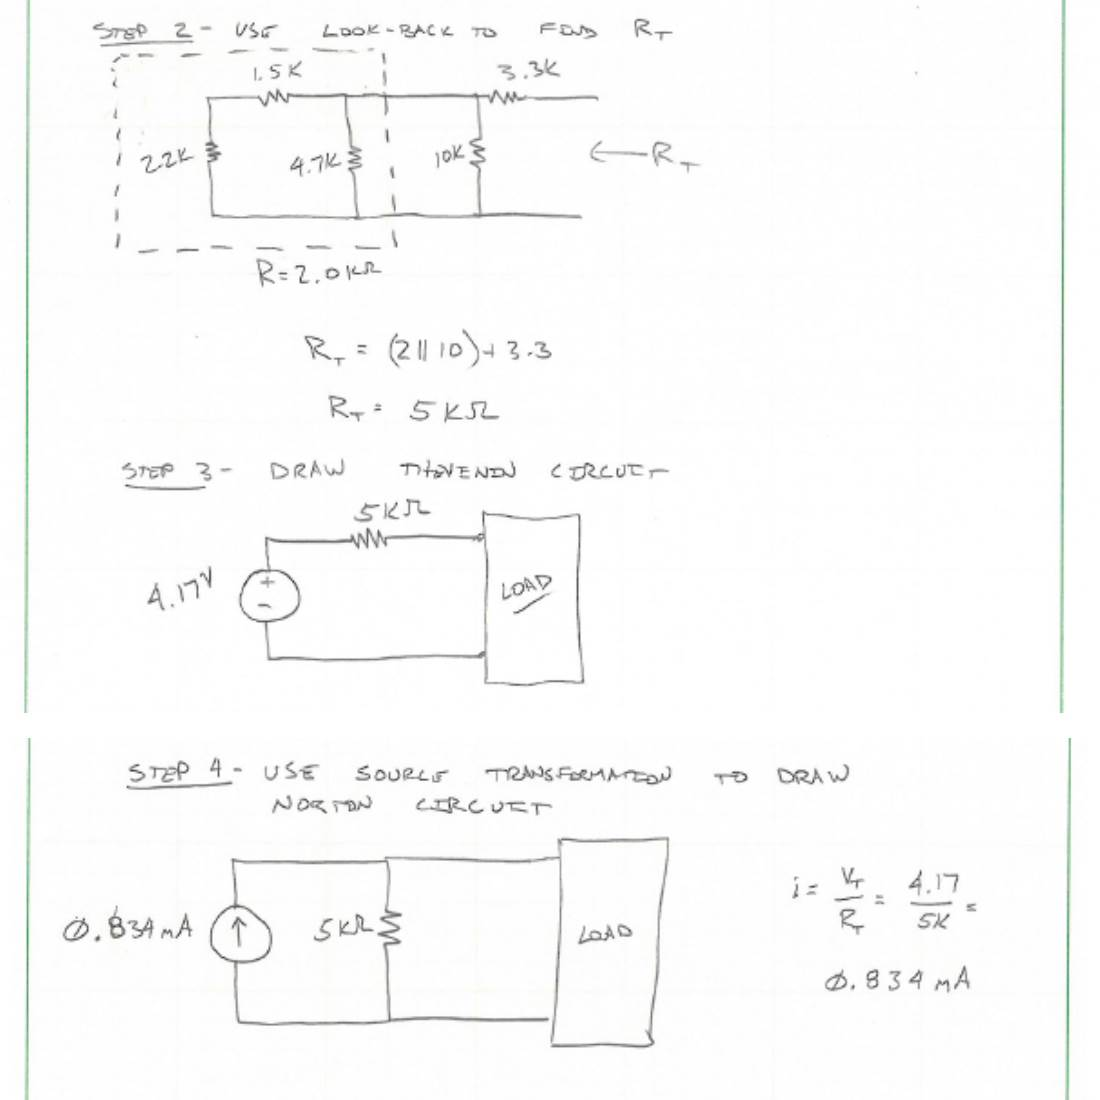
\includegraphics[width=0.9\textwidth]{Example1solnB.jpg}
\end{figure}
}

\newpage
\clearpage
\pagebreak


\subsection{Example 2 - Textbook Exercise 3-30}
Find the Thevenin and Norton equivalents of the circuit shown in Figure \ref{fig: Example2}.  Then find the voltage, current and power delivered to a $50 \Omega$ load. 
\begin{figure} [h t b]
\centering
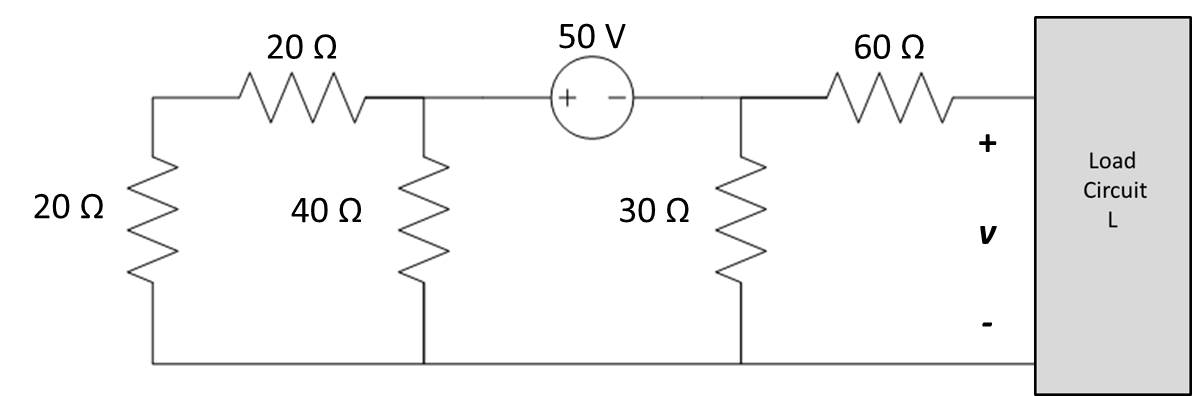
\includegraphics[width=0.7\textwidth]{Example2.jpg}
\caption{Example 2 Circuit}
\label{fig: Example2}
\end{figure}

\soln{6in}{
\begin{figure} [h t b]
\centering
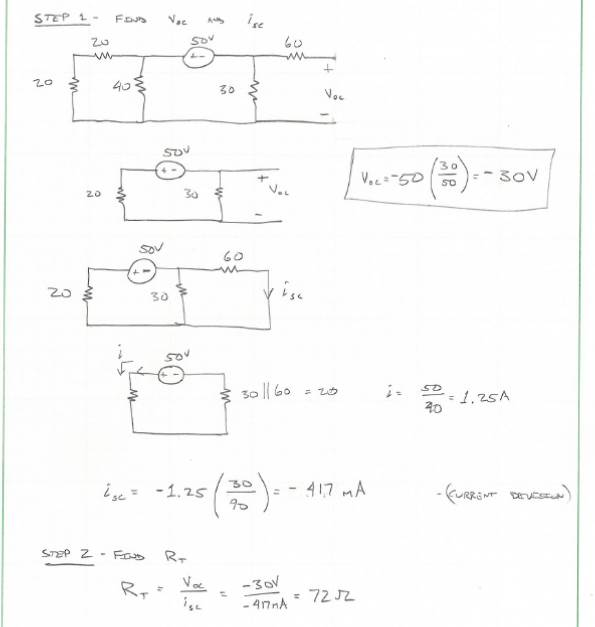
\includegraphics[width=0.7\textwidth]{Example2solnA.jpg}
\end{figure}

\begin{figure} [h t b]
\centering
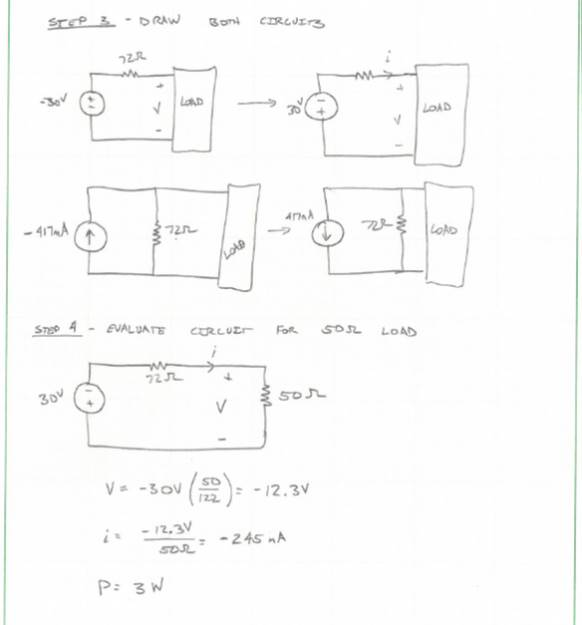
\includegraphics[width=0.9\textwidth]{Example2solnB.jpg}
\end{figure}
}

\newpage
\clearpage
\pagebreak

\subsection{Example 3 - Textbook Exercise 3-31}
Find the current and power delivered to an unknown load in Figure \ref{fig: Example2} if $v=+6\ V$ . 

\soln{6in}{
\begin{figure} [h t b]
\centering
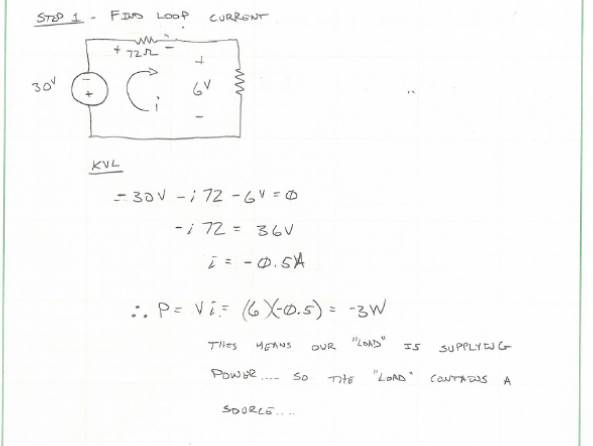
\includegraphics[width=0.9\textwidth]{Example3soln.jpg}
\end{figure}
}

\newpage
\clearpage
\pagebreak

\subsection{Example 4}
Use Thevenin's theorem to find $v_o$ in Figure \ref{fig: Example4} 
\begin{figure} [h t b]
\centering
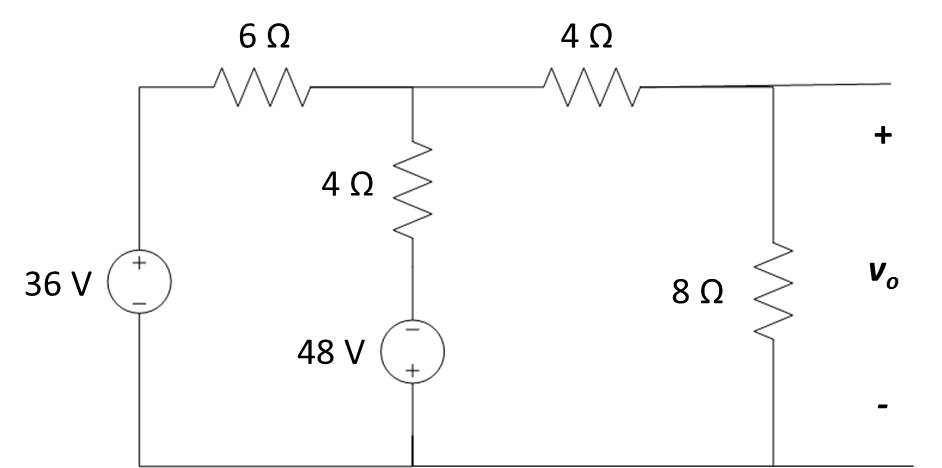
\includegraphics[width=0.7\textwidth]{Example4.jpg}
\caption{Example 4 Circuit}
\label{fig: Example4}
\end{figure}

\soln{6in}{
\begin{figure} [h t b]
\centering
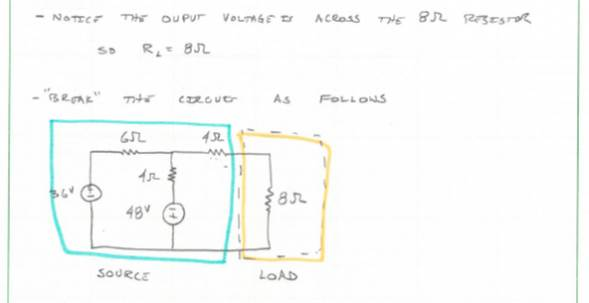
\includegraphics[width=1\textwidth]{Example4solnA.jpg}
\end{figure}

\begin{figure} [h t b]
\centering
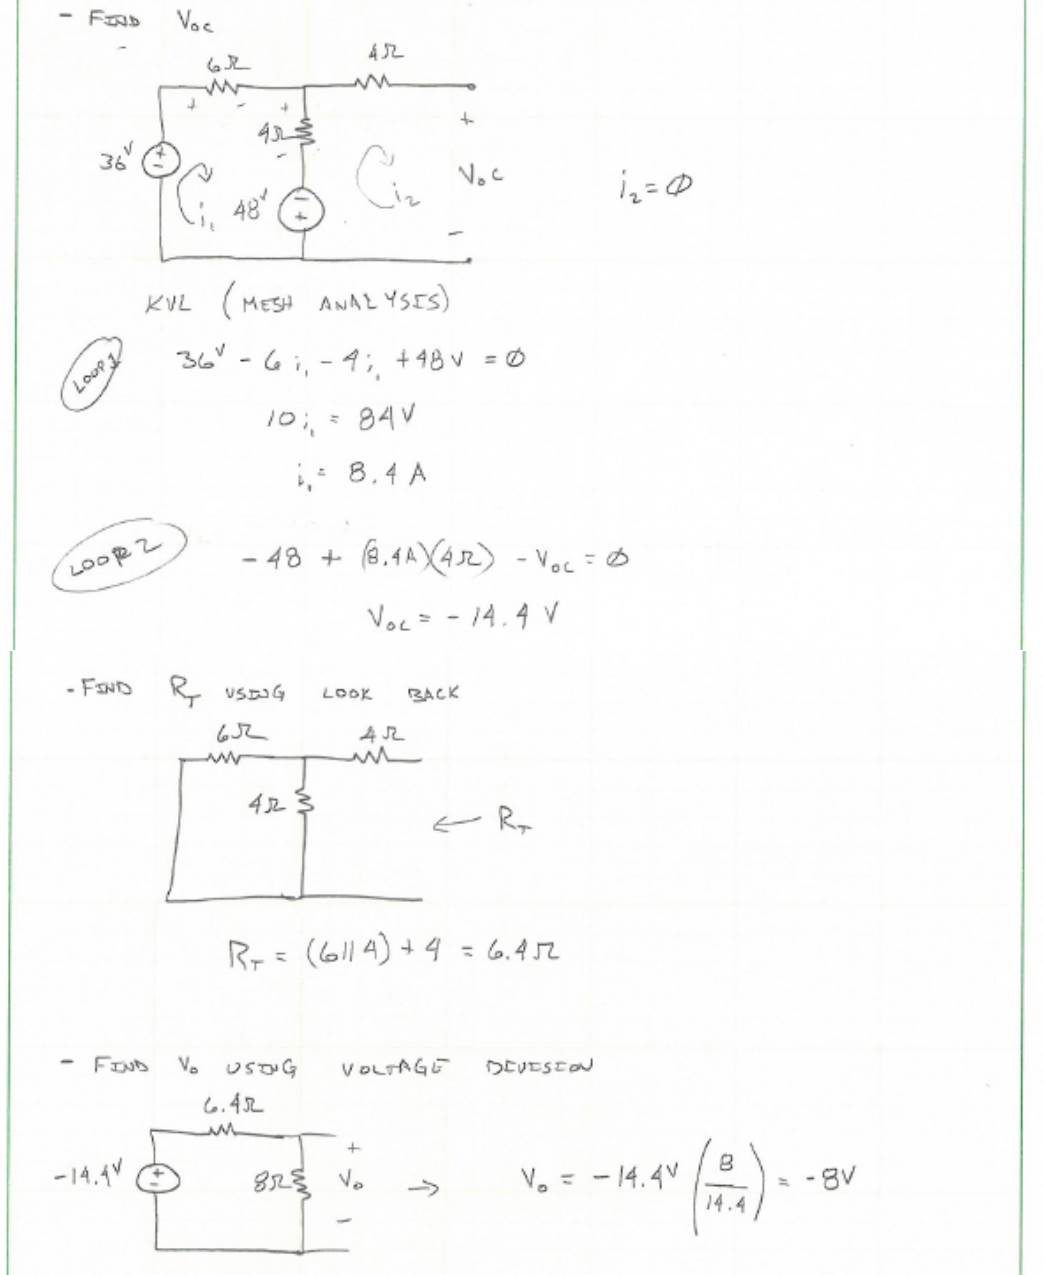
\includegraphics[width=1\textwidth]{Example4solnB.jpg}
\end{figure}
}

\newpage
\clearpage
\pagebreak

\subsection{Example 5}
Use Norton's theorem to find $v_o$ in Figure \ref{fig: Example5} 
\begin{figure} [h t b]
\centering
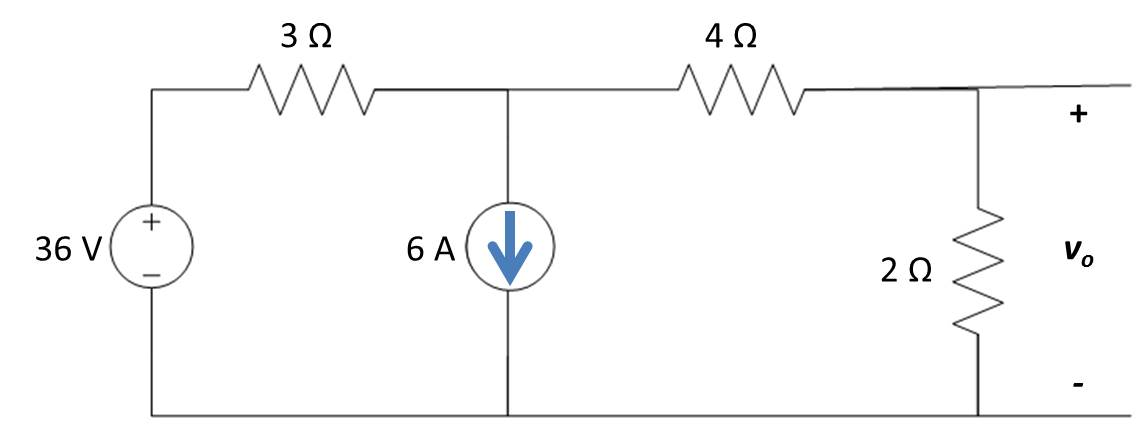
\includegraphics[width=0.7\textwidth]{Example5.jpg}
\caption{Example 5 Circuit}
\label{fig: Example5}
\end{figure}

\soln{6in}{
\begin{figure} [h t b]
\centering
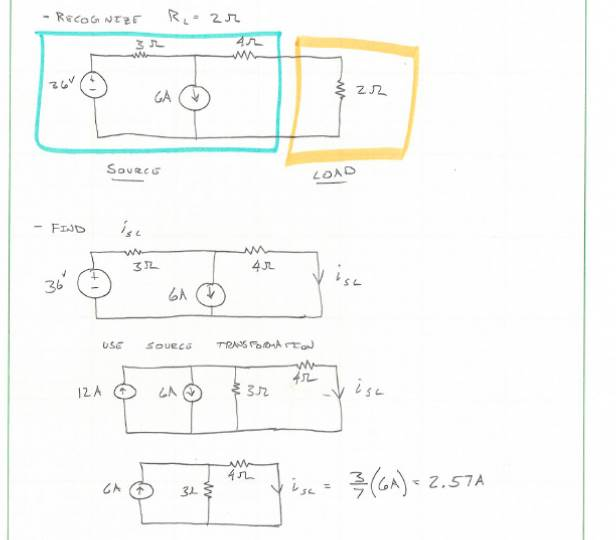
\includegraphics[width=0.8\textwidth]{Example5solnA.jpg}
\end{figure}

\begin{figure} [h t b]
\centering
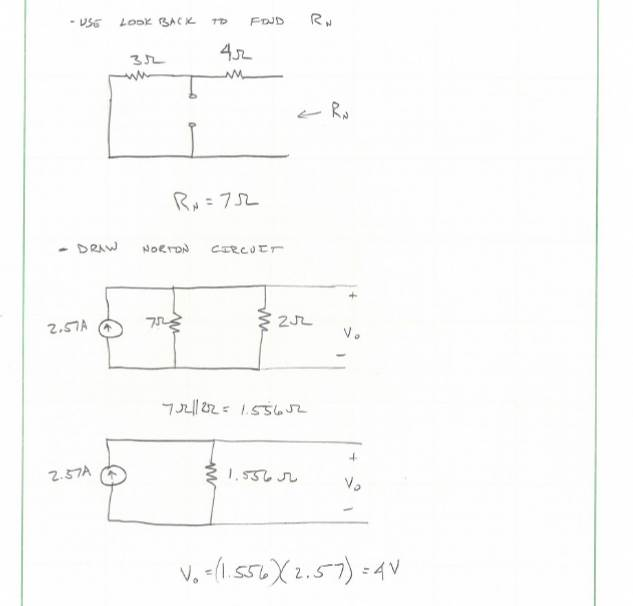
\includegraphics[width=1\textwidth]{Example5solnB.jpg}
\end{figure}
}

\newpage
\clearpage
\pagebreak

\end{document}


% Equation Array Example Code
%\begin
%{eqnarray}
%P_R &=& i_R^2R \nonumber \\
%P_R &=& (100\ mA)^2 \times 100\ \Omega \nonumber \\
%P_R &=& (100 \times 10^{-3}\ A)^2 \times 100\ \Omega \\
%P_R &=& 10000 \times 10^{-6}\ A^2  \times 100\ \Omega \nonumber \\
%P_R &=& 1\ W  \nonumber
%\end{eqnarray} 

% Figure Example Code
%\begin{figure} [h t b]
%\centering
%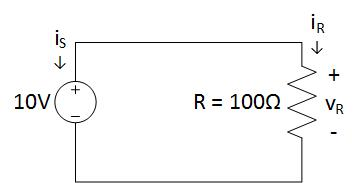
\includegraphics[width=0.5\textwidth]{OhmsLawExampleSolution.jpg}
%\caption{Ohm's Law example circuit}
%\label{fig: OhmsLawExampleSolution}
%\end{figure}

%Table Example Code
%\begin{table}[h]
%\centering
%\begin{tabular}{|l|c|c|}
%\hline
%Prefix & Abbreviation & Value \\
%\hline \hline
%Giga & $G$ & $10^9$ \\
%Mega & $M$ & $10^6$ \\
%Kilo & $k$ & $10^3$ \\
%\hline
%milli & $m$ & $10^{-3}$ \\
%micro & $\mu$ & $10^{-6}$ \\
%nano & $n$ & $10^{-9}$ \\
%pico & $p$ & $10^{-12}$ \\
%\hline
%\end{tabular}
%\caption{Engineering prefixes and values}
%\label{tab: Eng Prefixes}
%\end{table}
